\documentclass{tufte-handout}
\usepackage{amsmath}
\usepackage{amssymb}
\usepackage[protrusion,expansion=false,factor=1000,babel=false]{microtype}
\usepackage{enumitem}
\usepackage{booktabs}
\usepackage{algorithm}
\usepackage{algorithmic}
\usepackage{moreverb}
\usepackage{fancyvrb}
\fvset{fontsize=\normalsize}
\usepackage{tikz}
\usetikzlibrary{arrows,positioning,fit,decorations,decorations.pathmorphing,decorations.pathreplacing,calc,scopes,matrix}

\title{An API for Binary Code Parsing}
\author{Paradyn Parallel Performance Tools}

\begin{document}

\newcommand{\apient}[3]{%
#1 & #2 \\
 & \emph{#3} \\[0.5em]%
} 

\newenvironment{apilist}[1]{\begin{fullwidth}%
\begin{tabular}{p{0.25\linewidth}p{0.75\linewidth}}
{\bf #1} & \\%
}
{\end{tabular}\end{fullwidth}}


\maketitle


\section{Introduction}

\newthought{A binary code parser} converts the machine code representation of a
program, library, or code snippet to an abstraction of the instructions, basic
blocks, and functions that the binary code represents. The ParseAPI is a
multi-platform library for creating such abstractions from binary code sources.
The current incarnation uses SymtabAPI\cite{symtabsite} as the default binary
code source; all platforms and architectures handled by SymtabAPI are
supported. The ParseAPI is designed to be easily extensible to other binary
code sources. Support for parsing binary code in memory dumps or other formats
requires only implementation of a small interface as described in this
document.

This API provides the user with a control flow-oriented view of a binary code
source. Each code object such as a program binary or library is represented as
a top-level collection containing the functions, basic blocks, and edges that
represent the control flow graph. A simple query interface is provided for
retrieving lower level objects like functions and basic blocks through address
or other attribute lookup. These objects can be used to navigate the 
program structure as described below.

\subsection{Abstractions}

\begin{marginfigure}[2cm]
\centering
\begin{tikzpicture}[line width=1pt,x=\marginparwidth*.95/12,y=\marginparwidth*.95/12]

%\draw[help lines] (0,0) grid [step=1] (12,18) ;

 %cfg nodes

    \matrix (cfg1) [matrix of math nodes,
             column sep={0.33cm},
             row sep={0.6cm},
             nodes={circle, draw, minimum size=0.5cm}]
    {
               & |(n1)| b_1 &    \\
     |(n2)| b_2 &           & |(n3)| b_3 \\[1.1cm]
     |(n4)| b_4 &           &    \\
               & |(n5)| b_5 &    \\
    };

    \matrix [matrix of math nodes,
             column sep={0.33cm},
             row sep={0.6cm},
             nodes={circle, draw, minimum size=0.5cm},
             below right=-3.5 and -1 of cfg1]
    {
               & |(m1)| b_6 &    \\
     |(m2)| b_7 &           & |(m3)| b_8 \\
               & |(m4)| b_9 &    \\
    };

    \begin{scope}[>=stealth,->,looseness=0.5,auto,
        every node/.style={font=\scriptsize\itshape}]
        \draw (n1) to [bend right] (n2) ;
        \draw (n1) to [bend left] (n3) ;
        \draw (n2) to [bend left] (n4) ;
        \draw (n4) to [bend left] (n2) ;
        \draw (n4) to [bend right] (n5) ;
        \draw (n3) to [bend left] (n5) ;
        \draw (m1) to [bend right] (m2) ;
        \draw (m1) to [bend left] (m3) ;
        \draw (m2) to [bend right] (m4) ;
        \draw (m3) to [bend left] (m4) ;
        % call
        \draw [dotted] (n3) to [bend left] node [midway] {call} (m1) ;
    \end{scope}
\end{tikzpicture}
\caption{The control flow graph of two functions joined by an interprocedural \emph{call} edge.}
\end{marginfigure}

\newthought{The basic representation} of code in this API is the control flow
graph. The nodes of the CFG represent basic blocks: straight-line sequences of
instructions $I_i \ldots I_j$ where for each $i < k \le j$, $I_k$ postdominates
$I_{k-1}$. The typed edges between nodes in the graph represent execution
control flow, such as conditional and unconditional branches, fallthrough
edges, and calls. The graph therefore represents both \emph{inter-} and
\emph{intraprocedural} control flow: traversal of nodes and edges can cross the
bounaries of the higher level abstractions like \emph{functions}. Such
abstractions can nonetheless be obtained using this API.  A function represents
the set of all blocks reachable from a \emph{function entry point} through
intraprocedural control flow only. The entry points of functions are determined
by the parser library through various means, such as hints from debugging
symbols and recursive traversal along call edges.

\subsection{Interfaces}

The following classes define the publicly visible interfaces of the ParseAPI:

\begin{itemize}[label=$\circ$]
{\item {\sc codeobject}: represents the parsed form of a binary code object,
such as a program binary or library. Provides query access to CFG constructs
such as functions and basic blocks.}

{\item {\sc function}: represents a function and information about it, such as
its entry address, the list of blocks reachable through intraprocedural control
transfers, or whether the function is known to never return.}

{\item {\sc block}: represents a basic block, its start and end point, and control edges between the block and its successors and predecessors.}

{\item {\sc edge}: represents a control flow edge.}
\end{itemize}

\noindent
This API is meant to be extensible: with the exception of the CodeObject, all
of the default classes above can be extended to form the basis of some richer
abstraction over program control flow. Additionally, this API can be easily
applied to various code sources. The following interfaces are provided to
support extension to binary code sources besides those supported by the
SymtabAPI.

\begin{itemize}

{\item {\sc instructionsource}: represents an object from which pointers to machine instructions can be obtained. An InstructionSource implements a minimal contract as specified in the API details below.}

{\item {\sc codesource}: represents a binary code object. A CodeSource provides
access to the binary code through an InstructionSource, and optionally provides
a list of \emph{hints} that suggest starting locations for parsing, as well as
other binary characteristics like external linkage. For example, the provided
SymtabCodeSource specialization re-exports function symbols as hints for
parsing.}

{\item {\sc cfgfactory}: a factory for Function, Block, and Edge objects. A default allocator for these objects is provided. To use the parser with specialized extensions of the CFG objects, a custom CFGFactory that knows how to allocate such objects must implement the minimal contract of this interface.}

\end{itemize}

\section{A Simple Example}

The code example below illustrates how the ParseAPI can be used alongside of
the SymtabAPI to print out the control flow graph for a program binary.
\begin{listing}[1]{1}
using namespace Dyninst;
using namespace Dyninst::ParseAPI;

vector<Function *> funcs;

SymtabCodeSource * sts = new SymtabCodeSource("foobinary");
CodeObject * co = new CodeObject(sts);
\end{listing}
\noindent
Once the binary has been loaded (in this case using a SymtabAPI object as the
sbinary code source), it can be parsed and all of the functions can be
retrieved. The list of blocks reachable from each function can be retrieved
and output.\footnote{Alternatively, the intraprocedural control flow graph
for each function could be traversed starting with its first block by not
following \emph{call} edges.}

\begin{listingcont}
co->parse();

int cnt = co->allFuncs(funcs);
for(int i=0;i<fcnt;++i) {
    const vector<Block *> & blocks = funcs[i]->blocks();
    for(unsigned j=0;j<blocks.size();++j) {
        vector<Edge *> & targets = blocks[j]->targets();
        for(unsigned k=0;k<targets.size();++j) {
            // print out block -> target
        }
    }
}
\end{listingcont}

\section{API Reference}

There are two major sections of the public API. The first is the CodeObject and
the CFG objects it provides access to; these represent the parsed program
binary. The second section is the interfaces necessary to extend the ParseAPI
to new binary code sources or to support specializations of the CFG objects.

\subsection{CFG Objects}

\begin{apilist}{CodeObject}
\apient{}{CodeObject(CodeSource * cs, CFGFactory * fact = NULL)}{Constructs a new CodeObject. The CodeSource argument is mandatory; if the CFGFactory argument is not provided, a default factory is used.}
\apient{void}{parse()}{Parses the binary code object using the default hint-based and recursive traversal algorithm.}
\apient{Function *}{findFuncByEntry(Address entry)}{Returns a pointer to the function starting at the given address or NULL.}
\apient{int}{findFuncs(Address addr, set<Function*> \& funcs)}{Finds all functions overlapping the given address, returning the number found.}
\apient{int}{allFuncs(set<Function*> \& funcs)}{Places all known functions in the provided set, returning the total number.}
\apient{int}{findBlocks(Address addr, set<Block*> \& blocks)}{Finds all blocks overlapping a given point. Blocks are allowed to overlap, as is possible on architectures with variable-length instruction sets.}
\apient{bool}{findCatchBlock(Address addr, Address \& catchStart)}{Finds the exception catch block covering the provided address, filling its starting point into catchStart if it exists.}
\apient{bool}{non\_returning(Address func\_entry)}{Queries CodeSource for known non-returning status of the function starting at func\_entry.}
\apient{bool}{non\_returning(string func\_name}{Queries CodeSource for known non-returning status of the named function.}
\end{apilist}

\begin{apilist}{Function}
\apient{}{Function(Address addr, CodeObject \& obj)}{Function constructor. The ParseAPI never calls this routine explicitly, instead using the CFGFactory mkfunc() method to allocate an object of the appropriate subclass.}
\apient{const char *}{name()}{Returns the name of the function.}
\apient{Address}{addr()}{Returns the function entry address.}
\apient{vector<Block *> \&}{blocks()}{Returns a reference to the vector of blocks reachable through intraprocedural control flow from this function entry point.}
\end{apilist}

\begin{apilist}{Block}
\apient{}{Block(Address start)}{Block constructor.}
\apient{Address}{start()}{Returns block start address.}
\apient{Address}{end()}{Returns block end address.}
\apient{Address}{last\_insn()}{Returns address of last instruction.}
\apient{Address}{size()}{Returns end() - start().}
\apient{vector<Edge*> \&}{sources()}{Returns vector of predecessor blocks in the control flow graph.}
\apient{vector<Edge*> \&}{targets()}{Returns vector of successor blocks in the control flow graph.}
\end{apilist}

\begin{apilist}{Edge}
\apient{}{Edge(Block * source, Block *target, EdgeTypeEnum type)}{Constructor.}
\apient{Block *}{src()}{Returns source component of this edge.}
\apient{Block *}{trg()}{Returns type component of this edge.}
\apient{EdgeTypeEnum}{type()}{Returns the edge type.}
\end{apilist}

\subsection{Extension Interface}

\begin{apilist}{CodeSource}
\apient{InstructionSource *}{isrc()}{Returns a pointer to an instruction source implementation. (implementation mandatory)}
\apient{vector<hint\_t> *}{hints()}{Returns a pointer to a vector of (location,name) pairs of function entry hints, or NULL if no such hints are provided by this code source. (implementation optional)}
\apient{bool}{non\_returning(Address func\_entry)}{Checks known non-returning status of the function starting at func\_entry. (implementation optional)}
\apient{bool}{non\_returning(string func\_name}{Checks known non-returning status of the named function. (implementation optional)}
\apient{map<Address,string> \&}{linkage()}{Returns external linkage map. (implementation optional)}
\end{apilist}

\begin{apilist}{InstructionSource}
\apient{bool}{isValidAddress(Address)}{}
\apient{void*}{getPtrToInstruction(Address)}{}
\apient{void*}{getPtrToData(Address)}{}
\apient{unsigned int}{getAddressWidth()}{}
\apient{bool}{isAligned(Address)}{}
\apient{bool}{isCode(Address)}{}
\apient{bool}{isData(Address)}{}
\apient{Address}{codeOffset()}{}
\apient{Address}{codeLength()}{}
\end{apilist}

\begin{apilist}{CFGFactory}
\apient{Function *}{mkfunc(Address addr, FuncSource src, CodeObject \& obj)}{}
\apient{Block *}{mkblock(Function * f, Address addr)}{}
\apient{Edge *}{mkedge(Block *src, Block *trg, EdgeTypeEnum type)}{}
\apient{void}{free\_func(Function *f)}{}
\apient{void}{free\_block(Block *b)}{}
\apient{void}{free\_edge(Edge *e)}{}
\apient{void}{free\_all()}{}
\end{apilist}


\bibliographystyle{plainnat}
\nobibliography{parseapi}

\end{document}
